% !TeX spellcheck = <none>
\documentclass[11pt,a4paper,twoside]{article}
\usepackage{a4wide}	% für gut definierte Seitenränder und Platzausnutzung
\usepackage[utf8]{inputenc}	% für Umlaute
\usepackage{amssymb,amsmath}
\usepackage{booktabs}   % schöne Tabellen
\usepackage[pdftex]{graphicx}
\usepackage{epstopdf}
\usepackage{siunitx}	% für SI-Einheiten; siehe http://mirror.unicorncloud.org/CTAN/macros/latex/contrib/siunitx/siunitx.pdf
\usepackage[version=3]{mhchem}	% chemische Symbole mit \ce{}
\usepackage{listings} 	% für Einbinden von Quellcode
\usepackage{color}	% für das Einfärben von eingebundenem Quellcode
\usepackage{longtable}	% für das Erstellen mehrseitiger Tabellen
\usepackage[german]{isodate} % Datumformatierung für \today
\usepackage{marvosym}


% declaring custom units
\DeclareSIUnit \mag {mag} 
\DeclareSIUnit \parsec {pc}
\DeclareSIUnit \AU {AU}

% format angle display
\sisetup{add-arc-degree-zero}
\sisetup{add-arc-minute-zero}
\sisetup{add-arc-second-zero}
\sisetup{arc-separator = \,}


%Befehl, um Quellcode einzufügen: 
%\lstinputlisting[caption = {``title``}, captionpos = b, language=C++]{data.cpp}

%Befehl, um Graphik einzufügen:   
%\begin{figure}
%  \centering
%  \includegraphics[width=0.7\textwidth, angle=-90]{center_diff.eps}
%  \caption{centered differencing at t = 4}
%\end{figure}

% Befehl für kein ``\noindent mehr''
\setlength\parindent{0pt}

%\lstset{numbers=left}

\newcommand{\op}[1]{\operatorname{#1}}

% Konsistente Variablennamen:
\newcommand{\zen}{\ensuremath{\nu} }    % zenith angle
\newcommand{\hei}{\ensuremath{h} }      % height angle
\newcommand{\HA}{\ensuremath{\Gamma} }  % hour angle \HA
\newcommand{\DEC}{\ensuremath{\delta} } % declination \DE
\newcommand{\LAT}{\ensuremath{\Phi} }   % latitude \LAT
\newcommand{\electron}{\ce{e^-}}
\newcommand{\SNR}{\ensuremath{\frac{S}{N}} }

\lstset{
   basicstyle=\scriptsize\ttfamily,			% grundlege des Design
   keywordstyle=\ttfamily,				% Design von Schlüsselwörtern (Codebefehle wie Variablentypen, Schleifenbefehle u.Ä.)
   stringstyle=\ttfamily,				% Design von Variablen
   commentstyle=\ttfamily\color{blue},			% Design von Kommentaren
   showstringspaces=false,				% Leerzeichen in Strings darstellen?
   flexiblecolumns=false,				% dynamische Spaltenbreite?
   tabsize=2,						% Länge des Tabulators
   % Einstellung der Zeilennummerierung:
   numbers=left,					% Position der Nummern
   numberstyle=\tiny,					% Größe der Nummern
   numberblanklines=true,				% Leerzeilen durchnummerieren?
   numbersep=20pt,					% Platz zwischen Nummern und Code
   xleftmargin=30pt					% Platz zum linken Seitenrand
 }
 
%opening
\title{\LARGE \underline {Sheet 5}}
\author{Johannes Haux \\ Florian Trost \\ Elsa Wilken}
\date{\today}


\begin{document}

\maketitle
\thispagestyle{empty}

\begin{center}
  Astronomical Techniques (MKEP5) \\
  \baselineskip35pt
  by Prof. Dr. Stefan Wagner and Priv.-Doz. Dr. Thorsten Lisker \\
  \baselineskip60pt
  Ruprecht Karl University of Heidelberg
\vskip 40pt
%
\includegraphics[width=5cm]{pic/UniHD.png}

\end{center}

\newpage
\setcounter{page}{1}		% set page count to start with 1 here
\section*{Exercise A.}
In the lectures of May 31 and June 2 you have reduced (i.e. corrected for
bias, flat-field, and subtracted the sky background emission) and calibrated in wavelength
the spectrum of the spiral galaxy NGC 3263 shown in Fig. 1.\\
\subsection*{1.} What is the dispersion (\AA/pixel) of grating \#6 (through which the spectrum was taken) as
you derived from the wavelength calibration? (1 points)
\subsection*{2.}
What is the resolution (\AA) of grating \#6? To compute it, you need to measure the
gaussian Full Width Half Maximum (gFWHM) of the emission lines in the arc lamp
spectrum. Set the parameter nsum = 10 and dispaxis = 2 in the IRAF routine
ONEDSPEC, and plot the spectrum of the arc lamp with SPLOT whose parameter line is
258. Choose an emission line in the plotted spectrum and press “k” on the closest
continuum point to the left of the line and press “k” again on the closest continuum point to
the right of the line. This corresponds to fitting a gaussian profile to the chosen line, and
the gaussian parameters (peak wavelength, integrated flux, equivalent width=eqw and
gfwhm) appear on the bottom of the graphical iraf term window. (2 points)\\
\textbf{Answer}\\
We followed the instructions on the homework sheet (See \ref{fig:A2_gausssfit}). So we got an gaussian fit of a certain emission line with the following gfwhm:
\begin{equation*}
gfwhm=\SI{3.314}{\angstrom}
\end{equation*}
This is the resolution.
\begin{figure}[h]
\centering
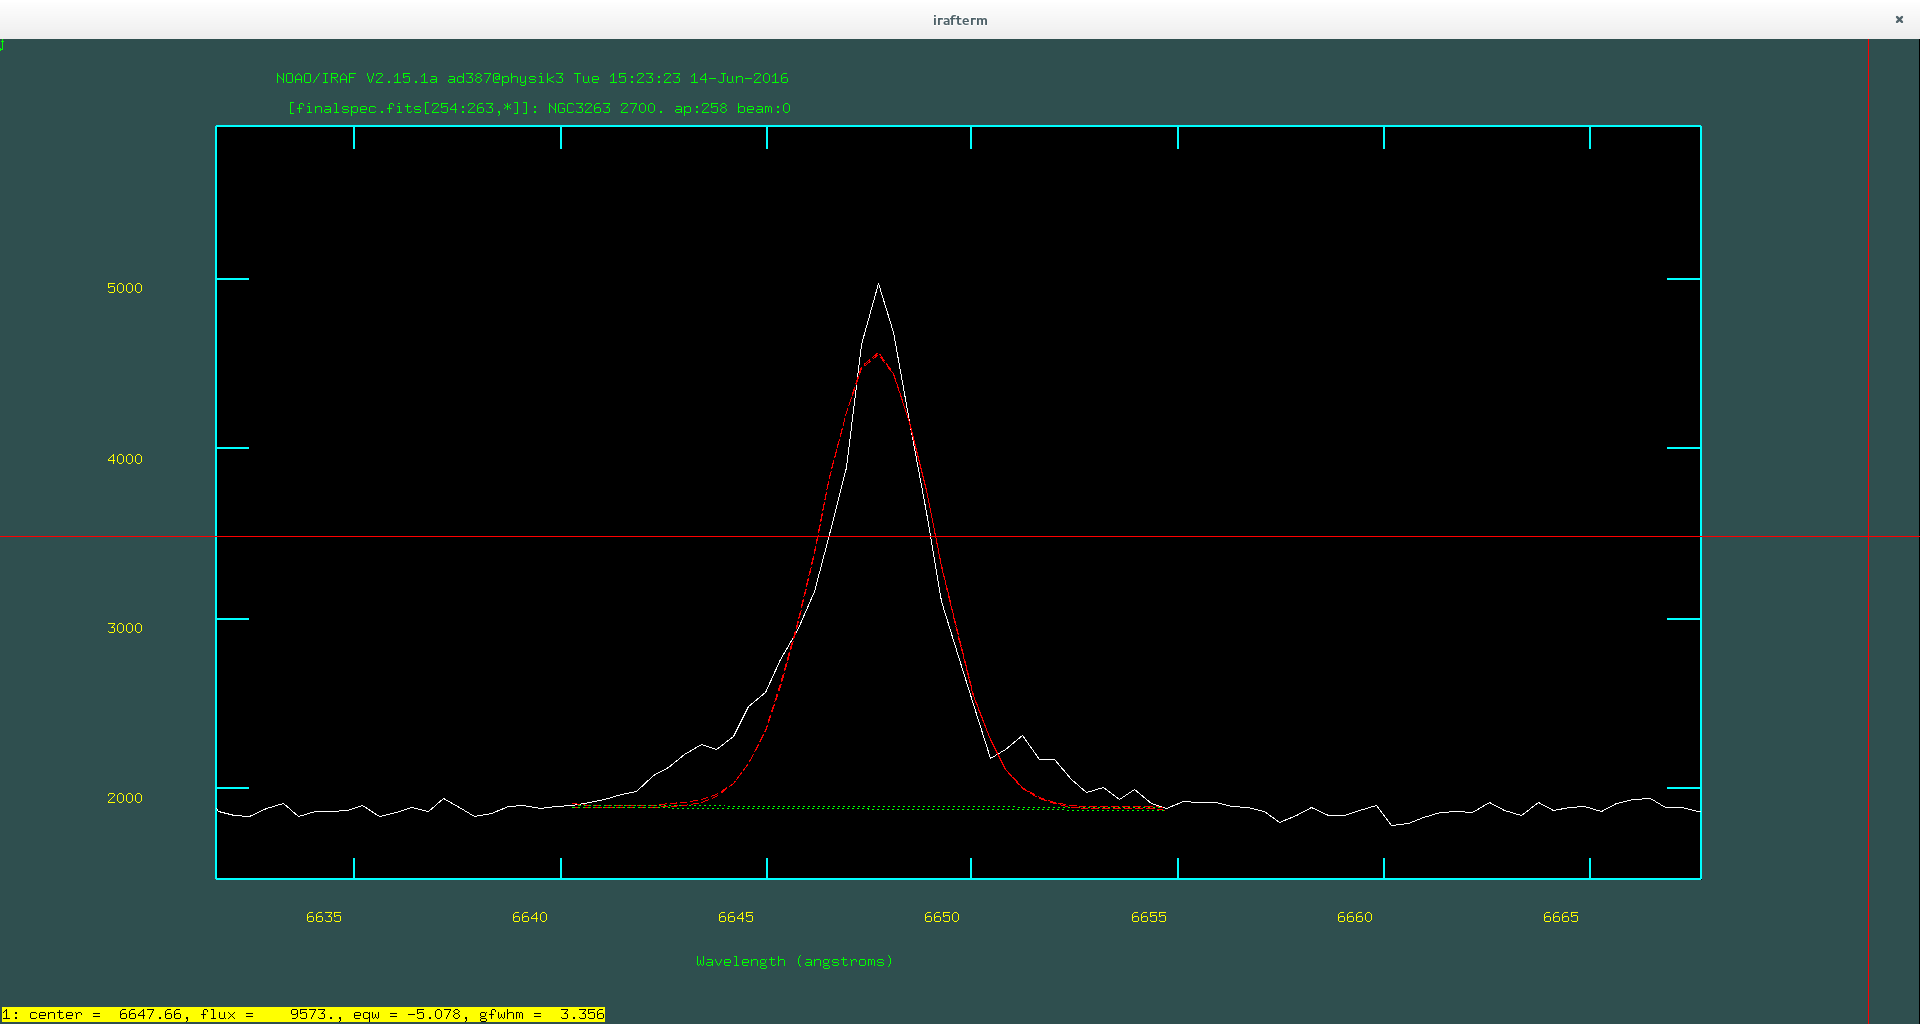
\includegraphics[width=0.7\linewidth]{pic/A2_gausssfit}
\caption{}
\label{fig:A2_gausssfit}
\end{figure}

\subsection*{3.} The slit used in these observations has a width of 1 arcsec. Would the resolution that
you just measured above change if the slit were larger or narrower? (1 points)\\

\textbf{Answer}\\
For a larger slit the resolution would decrease. 
\subsection{4.}
Use SPLOT and the option “e” to measure the peak wavelength of the Halpha emission
at different spatial positions. You need to place the cursor on the closest continuum point
to the left of the line and press “e”. Then, place the cursor again on the closest continuum
point to the right of the line and press “e” again. This will allow you to measure the centroid
wavelength of the line which is called “center” and will appear on the bottom of the
graphical iraf term window.
Compute the radial velocity of the Halpha line from the centroid wavelength keeping in
mind that the rest-frame wavelength of the Halpha emission is 6562.82 Å in air. In this
case, set nsum = 20 in ONEDSPEC, use SPLOT with line = 55 and measure the centroid
wavelength of the Halpha line with the “e” option. Re-iterate the same procedure for
different values of line, i.e. 75, 95, 115 .... 355. The galaxy centre is at pixel X G = 258;
compute the distance d = (line value – X G ) of each measurement of the Halpha from the
galaxy centre, and transform this distance in arcsec (using the pixel scale given in Fig. 1).
Now you are ready to plot the radial velocity of each measurement as a function of
distance from the galaxy centre, also known as the rotation curve of a spiral galaxy.
Please, submit your plot with your other solutions. (9 points)\\
\textbf{Answer}\\
We followed the instructions on the homework sheet. \\
Calculation of the Distance:
\begin{equation*}
d = (line\,value – X_G )
\end{equation*}
With $X_G$=258\\
line value: 55-335\\ 
Calculation of the Radial velocitys v from the wavelength:
\begin{equation*}
 v=\left( \frac{\lambda}{\SI{6562.82}{\angstrom}}-1\right) \cdot speed\,of\,light
\end{equation*}
To  measure the peak wavelength of the Halpha emission at different spatial positions we tried to find the peak at different lines of finalspec. We are not sure if we measuered every time the right emission line, so we got probably a rather large error.\\

\begin{figure}[h!]
\centering
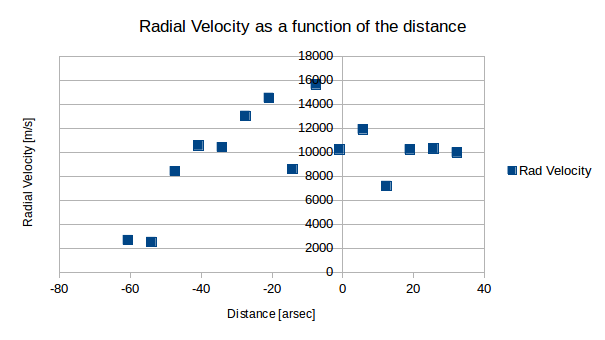
\includegraphics[width=1\linewidth]{pic/Radial_velocity}
\caption{}
\label{fig:Radial_velocity}
\end{figure}
In figure \ref{fig:Radial_velocity} the results of our messurements are shown.

\end{document}
%Helgoland05042703#